\documentclass[12pt,a4paper]{article}
\usepackage[T1]{fontenc}
\usepackage[utf8]{inputenc}
\usepackage[indonesian]{babel}
\usepackage{lmodern,geometry,graphicx,booktabs,array,float,microtype}
\usepackage{amsmath,amssymb}
\usepackage{algorithm,algpseudocode,listings}
\usepackage[hidelinks]{hyperref}
\geometry{margin=2.54cm}
\emergencystretch=1em
\numberwithin{equation}{section}
\counterwithin{table}{section}
\counterwithin{figure}{section}
\counterwithin{algorithm}{section}
\floatname{algorithm}{Kode}
\renewcommand{\lstlistingname}{Kode}
\algrenewcommand\algorithmicrequire{\textbf{Masukan:}}
\algrenewcommand\algorithmicensure{\textbf{Keluaran:}}
\newcommand{\R}{\mathbb{R}}
\newcommand{\norm}[1]{\left\lVert #1\right\rVert_2}
\lstset{language=Python,basicstyle=\ttfamily\footnotesize,breaklines=true,
  columns=fullflexible,keepspaces=true,showstringspaces=false,frame=single}
\begin{document}
\setcounter{page}{2}
\begin{center}
{\large\bfseries TK 1: Sistem Persamaan Linear dan Least Square Problem}\par\medskip
Kelompok A12 -- Semester Gasal 2026/2027
\end{center}
\setcounter{tocdepth}{1}
\tableofcontents
\clearpage
\begin{center}{\large\bfseries Laporan 1: Analisis Perpindahan Penumpang Antarhalte}\end{center}
\addcontentsline{toc}{part}{Laporan 1: Analisis Perpindahan Penumpang Antarhalte}
\section*{Rangkuman}
Enam matriks transisi kode B untuk $N=16,32,64,128,256,512$ dipakai untuk menghitung distribusi stasioner penumpang. Sistem asal singular; satu persamaan diganti dengan syarat skala dan solusinya dinormalkan. Kami membandingkan LU dense berpivot parsial dengan eliminasi pita berpivot parsial untuk $p=2,q=1$. Pada $N=512$, solver pita memerlukan 20.09~ms dan 60~KiB, dibandingkan 164.22~ms dan 4108~KiB untuk dense. Kedua metode memberikan solusi dan residual yang sama pada ketelitian yang diamati. Kasus $N=256$ hampir terpisah menjadi dua blok dan memiliki kondisi terbesar, $\kappa_1(B)\approx1.71\times10^9$. Halte terakhir memiliki proporsi terbesar pada setiap ukuran. Untuk koridor besar, solver pita unggul dalam waktu dan memori, tetapi kondisi matriks tetap perlu dipantau.

\section{Pendahuluan dan Validasi Data}
Misalkan $X_k$ adalah halte penumpang pada interval ke-$k$ dan $T_{ij}=\Pr(X_{k+1}=j\mid X_k=i)$. Untuk setiap $N$, matriks $T$ dibaca dari CSV kode B yang sesuai dengan kelompok genap A12. Validasi memeriksa bentuk $N\times N$, elemen hingga dan nonnegatif, jumlah tiap baris satu hingga toleransi $10^{-12}$, serta keterhubungan kuat graf transisi. Dua pencarian graf, pada arah asli dan balik, memastikan rantai \emph{irreducible}; elemen diagonal positif memastikan aperiodisitas~\cite{norris}. Kondisi ini memberi distribusi stasioner tunggal dan konvergensi dari kondisi awal mana pun. Semua matriks lolos. Galat jumlah baris maksimum hanya $2.22\times10^{-16}$; setiap baris mempunyai dua sampai empat elemen tak-nol pada offset $-1,0,1,2$. Kasus $N=256$ memiliki peluang lintas blok berorde $10^{-8}$, sehingga valid namun hampir terpisah.

\begin{table}[H]\centering\small
\caption{Validasi data kode B. Semua ukuran lolos uji dimensi, nonnegativitas, jumlah baris, irreducibilitas, dan aperiodisitas.}\label{tab:validasi-ringkas}
\begin{tabular}{rrrrr}\toprule
$N$ & Galat baris maks. & $\min T_{ii}$ & $\min\{T_{ij}>0:i\ne j\}$ & Valid\\\midrule
16 & $1.11\times10^{-16}$ & 0.835 & 0.01442 & Ya\\
32 & $2.22\times10^{-16}$ & 0.835 & 0.01467 & Ya\\
64 & $2.22\times10^{-16}$ & 0.835 & 0.01483 & Ya\\
128 & $2.22\times10^{-16}$ & 0.835 & 0.01492 & Ya\\
256 & $2.22\times10^{-16}$ & 0.835 & $1.50\times10^{-8}$ & Ya\\
512 & $2.22\times10^{-16}$ & 0.835 & 0.01498 & Ya\\\bottomrule
\end{tabular}\end{table}
Tabel~\ref{tab:validasi-ringkas} memperlihatkan mengapa ukuran 256 perlu perhatian khusus: probabilitas perpindahan positif terkecil jauh lebih kecil daripada ukuran lain. Fungsi validasi juga diuji pada matriks kecil yang sengaja dibuat invalid, dan menolak nilai negatif, baris tidak stokastik, serta rantai yang tidak irreducible.

\section{Formulasi Sistem dan Struktur Pita}
Untuk vektor kolom proporsi $\pi^{(k)}$, hukum peluang total memberi $\pi^{(k+1)}=T^\mathsf{T}\pi^{(k)}$. Pada keadaan stasioner, $T^\mathsf{T}\pi=\pi$, $\mathbf1^\mathsf{T}\pi=1$, dan $\pi_i\ge0$. Dengan $A=I-T^\mathsf{T}$ diperoleh $A\pi=0$. Karena $T\mathbf1=\mathbf1$, maka $\mathbf1^\mathsf{T}A=0$: baris-baris $A$ bergantung linear dan $A$ singular. Baris pertama dapat diganti dengan syarat skala $z_1=1$:
\begin{equation}\label{eq:soal1-system}
B_{1,:}=e_1^\mathsf{T},\quad B_{i,:}=A_{i,:}\ (i\ge2),\quad b=e_1,\quad Bz=b,\quad \pi=\frac{z}{\mathbf1^\mathsf{T}z}.
\end{equation}
Untuk rantai irreducible, setiap keadaan akhirnya dapat mencapai halte 1; submatriks transisi di luar halte 1 memiliki jari-jari spektral kurang dari satu. Karena itu $B$ nonsingular~\cite{stewart}. Solusi $z$ belum berjumlah satu, sehingga normalisasi terakhir dalam~\eqref{eq:soal1-system} diperlukan.

Lower bandwidth $p=\max_{B_{ij}\ne0}(i-j)$ dan upper bandwidth $q=\max_{B_{ij}\ne0}(j-i)$ dihitung otomatis dengan memindai indeks semua entri tak-nol dan memperbarui kedua maksimum. Diperoleh $p=2,q=1$ untuk semua ukuran. Transposisi $T$ menukar offset $-1,0,1,2$ menjadi $1,0,-1,-2$; penggantian baris pertama dengan $e_1^\mathsf{T}$ tidak menambah elemen di luar pita. Jadi solver Thomas tridiagonal murni tidak berlaku. Penyimpanan dense membutuhkan $N^2$ bilangan, pita biasa $(p+q+1)N=4N$, dan pita dengan ruang \emph{fill-in} untuk pivoting $(2p+q+1)N=6N$ bilangan~\cite{golub,lapack}. Pada $N=512$ kebutuhan matriks dense 2~MiB, sedangkan array pita dengan \emph{fill-in} hanya 24~KiB.

\section{Dua Solver dan Uji Ukuran Kecil}
Kedua solver menyelesaikan $Bz=b$ lalu menerapkan normalisasi~\eqref{eq:soal1-system}. LU dense menyimpan faktor $L$ dan $U$ dalam satu array persegi. Pada langkah $k$, pivot dipilih sebagai indeks $r=\arg\max_{i\ge k}|B_{ik}|$, baris $k,r$ ditukar, multiplier $\ell_{ik}=B_{ik}/B_{kk}$ dihitung, dan sisa baris diperbarui. Permutasi baris ikut diterapkan ke $b$ sebelum substitusi maju dan balik, sehingga $PB=LU$~\cite{heath}. Solver pita memakai prinsip yang sama tetapi mencari pivot hanya pada baris $k,\ldots,k+p$ serta memperbarui kolom sampai $k+p+q$. Faktor disimpan sebagai diagonal pada array berukuran $(2p+q+1)\times N$; pertukaran dicatat sebagai vektor pivot. Ini merupakan perluasan algoritma Thomas untuk pita $p=2,q=1$ dengan pivoting.

\begin{algorithm}[H]
\caption{Langkah utama LU dense dan eliminasi pita berpivot parsial}\label{alg:soal1-solvers}
\begin{algorithmic}[1]
\Require $B$, $b$, serta bandwidth $p,q$ untuk mode pita
\State pilih mode dense atau simpan diagonal $B$ dalam array pita berukuran $(2p+q+1)\times N$
\For{$k=1,\ldots,N-1$}
  \State cari $r=\arg\max|B_{ik}|$ pada $i=k,\ldots,N$ (dense) atau $i=k,\ldots,\min(N,k+p)$ (pita)
  \State tukar baris aktif dan catat pivot; tolak sistem bila pivot nol
  \For{setiap baris aktif $i>k$}
    \State $\ell_{ik}\gets B_{ik}/B_{kk}$; perbarui entri setelah kolom $k$ dalam jangkauan mode
  \EndFor
\EndFor
\State terapkan pertukaran pada $b$; substitusi maju dan balik menghasilkan $z$
\State \Return $z/(\mathbf1^\mathsf{T}z)$
\end{algorithmic}
\end{algorithm}
Kode~\ref{alg:soal1-solvers} menunjukkan perbedaan jangkauan pivot dan pembaruan; algoritma linear utama diimplementasikan sendiri. Pada uji $B=\left(\begin{smallmatrix}2&1&1\\4&3&3\\8&7&9\end{smallmatrix}\right)$ dan $b=(3,7,19)^\mathsf{T}$, kedua solver memberi $z=(1,-1,2)^\mathsf{T}$ dan $\max|PB-LU|=0$. Uji rantai tiga halte dengan solusi $\pi=(1/4,1/2,1/4)^\mathsf{T}$ juga tepat. Pada keenam data soal, tidak terjadi pertukaran pivot dan selisih maksimum antardistribusi dari kedua solver adalah nol pada mesin pengujian. Pemanggilan solver pustaka hanya dipakai sebagai verifikasi terpisah.

\section{Waktu, Memori, dan Kompleksitas}
Pengukuran pada data soal dilakukan 15 kali per ukuran dan nilai minimum dilaporkan; waktu membaca CSV dipisahkan dari persiapan dan solver. Memori \texttt{.nbytes} mencakup array yang disimpan solver. Hasil pada Tabel~\ref{tab:bench-ringkas} menunjukkan titik silang di sekitar $N=128$: overhead perulangan Python membuat solver pita lebih lambat pada $N$ kecil, tetapi pada $N=512$ sekitar $8.2$ kali lebih cepat. Gambar~\ref{fig:waktu-ringkas} dan~\ref{fig:memori-ringkas} memperlihatkan tren waktu dan memori.
\begin{table}[H]\centering\small
\caption{Waktu solver minimum (ms) dan memori array solver (KiB) pada data soal.}\label{tab:bench-ringkas}
\begin{tabular}{rrrrr}\toprule
$N$ & Dense (ms) & Pita (ms) & Dense (KiB) & Pita (KiB)\\\midrule
16 & 0.310 & 0.544 & 4.4 & 1.9\\
32 & 0.678 & 1.104 & 16.8 & 3.8\\
64 & 1.527 & 2.235 & 65.5 & 7.5\\
128 & 4.500 & 4.512 & 259.0 & 15.0\\
256 & 18.041 & 10.179 & 1030.0 & 30.0\\
512 & 164.217 & 20.090 & 4108.0 & 60.0\\\bottomrule
\end{tabular}\end{table}
\begin{figure}[H]\centering
\includegraphics[width=.82\textwidth]{../soal1/hasil/waktu_vs_N.png}
\caption{Waktu solver terhadap jumlah halte; titik 1024 dan 2048 berasal dari data sintetis.}\label{fig:waktu-ringkas}
\end{figure}
\begin{figure}[H]\centering
\includegraphics[width=.82\textwidth]{../soal1/hasil/memori_vs_N.png}
\caption{Memori array solver terhadap jumlah halte pada data soal dan data sintetis.}\label{fig:memori-ringkas}
\end{figure}
LU dense membutuhkan $O(N^3)$ operasi dan $O(N^2)$ ruang. Untuk pita dengan pivoting, jangkauan operasi per langkah dibatasi sekitar $p(p+q)$, sehingga waktunya $O(Np(p+q))$ dan ruangnya $O(N(2p+q+1))$~\cite{golub}. Pada $p=2,q=1$, keduanya linear terhadap $N$. Eksperimen sintetis $N=2048$ memberi 12.68~s untuk dense dan 83.28~ms untuk pita, sesuai arah pertumbuhan tersebut. Input CSV sendiri dense, sehingga pembacaan dan deteksi pita dapat berbiaya $O(N^2)$ meskipun solvernya linear; penyimpanan awal sebagai diagonal menghilangkan hambatan ini.

\section{Kondisi, Galat, dan Interpretasi}
Seluruh eksperimen memakai $\kappa_1(B)=\|B\|_1\|B^{-1}\|_1$ agar norma kondisi konsisten. Residual $r=\|T^\mathsf{T}\pi-\pi\|_2$ dan galat normalisasi $e_{\rm norm}=|\mathbf1^\mathsf{T}\pi-1|$ dihitung setelah penyelesaian. Tabel~\ref{tab:kondisi-ringkas} menunjukkan kondisi sangat besar pada $N=256$ akibat penghubung antarblok yang amat kecil. Residual tetap kecil, tetapi residual kecil tidak menjamin galat maju kecil bila $B$ buruk kondisinya~\cite{higham}. Kedua solver memberi hasil identik pada data ini; galat maju terhadap acuan presisi tinggi pada $N=256$ sekitar $5.75\times10^{-11}$.
\begin{table}[H]\centering\small
\caption{Kondisi, residual, dan halte dengan proporsi maksimum; hasil kedua solver identik pada digit yang ditampilkan.}\label{tab:kondisi-ringkas}
\begin{tabular}{rrrrr}\toprule
$N$ & $\kappa_1(B)$ & $r$ & $e_{\rm norm}$ & Halte maks. ($\pi_i$)\\\midrule
16 & $1.68\times10^3$ & $1.55\times10^{-17}$ & 0 & 16 (0.09596)\\
32 & $6.52\times10^3$ & $1.30\times10^{-17}$ & 0 & 32 (0.04814)\\
64 & $2.57\times10^4$ & $9.66\times10^{-18}$ & 0 & 64 (0.02410)\\
128 & $1.02\times10^5$ & $5.95\times10^{-18}$ & 0 & 128 (0.01206)\\
256 & $1.71\times10^9$ & $3.85\times10^{-18}$ & 0 & 256 (0.00603)\\
512 & $1.62\times10^6$ & $3.21\times10^{-18}$ & 0 & 512 (0.00302)\\\bottomrule
\end{tabular}\end{table}
\begin{figure}[H]\centering
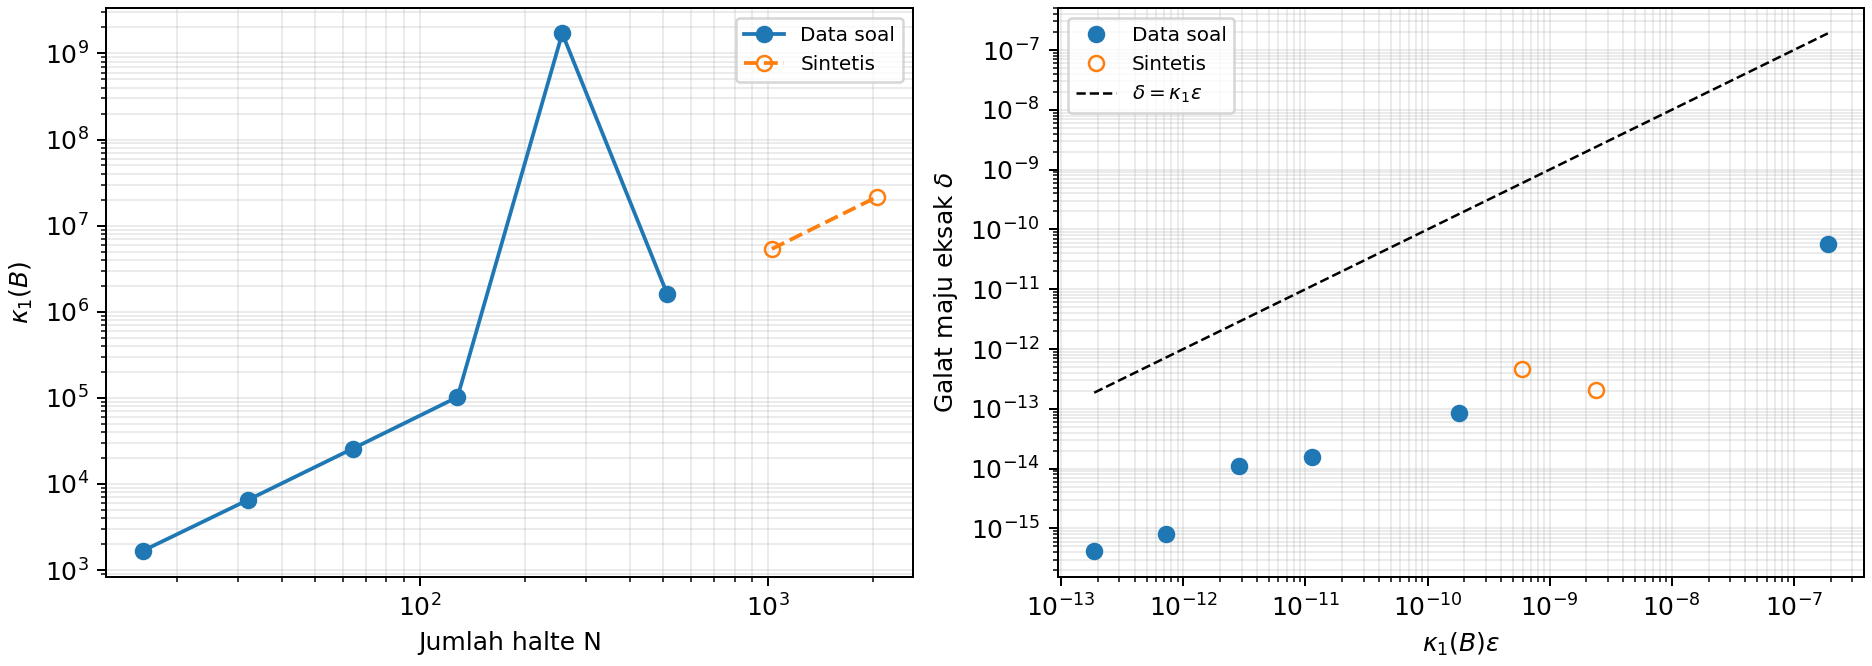
\includegraphics[width=.88\textwidth]{../soal1/hasil/kondisi_vs_N.png}
\caption{Bilangan kondisi terhadap $N$ dan galat maju terhadap batas kondisi.}\label{fig:kondisi-ringkas}
\end{figure}
\begin{figure}[H]\centering
\includegraphics[width=.88\textwidth]{../soal1/hasil/pi_vs_halte.png}
\caption{Profil distribusi stasioner terhadap nomor halte pada enam ukuran data.}\label{fig:pi-ringkas}
\end{figure}
Gambar~\ref{fig:kondisi-ringkas} menunjukkan lonjakan kondisi pada $N=256$, sedangkan Gambar~\ref{fig:pi-ringkas} memperlihatkan kenaikan $\pi_i$ ke arah ujung koridor. Halte terakhir memiliki proporsi terbesar pada keenam ukuran; pada $N=512$, $\pi_{512}\approx0.00301659$, sedangkan $\pi_1\approx0.00122645$. Massa menumpuk di ujung karena perpindahan maju tidak diimbangi oleh halte setelah $N$. Ini menunjukkan kebutuhan armada dan petugas relatif lebih tinggi di bagian akhir koridor; interpretasi tetap terbatas pada model transisi yang diberikan.

\section{Kesimpulan dan Rekomendasi}
Kedua solver akurat pada enam matriks uji. Solver pita adalah pilihan utama untuk jumlah halte besar karena memori dan operasi tumbuh linear pada lebar pita tetap, sedangkan LU dense tumbuh kuadratik dalam ruang dan kubik dalam waktu. Pemeriksaan $\kappa_1(B)$ tetap diperlukan: rantai hampir terpisah pada $N=256$ menunjukkan bahwa residual sangat kecil bisa menyertai sensitivitas solusi yang besar. Untuk data yang lebih buruk kondisinya, perbaikan iteratif atau algoritma GTH dapat dipertimbangkan~\cite{gth,higham}. Rekomendasi tersebut berdasarkan kompleksitas, waktu, memori, dan galat yang terukur; kedua teknik tambahan belum diuji di sini.

\clearpage
\begin{center}{\large\bfseries Laporan 2: Model SETAR untuk Prediksi Return Saham}\end{center}
\addcontentsline{toc}{part}{Laporan 2: Model SETAR untuk Prediksi Return Saham}
\setcounter{section}{0}
\section*{Rangkuman}
Kami membangun model SETAR dua rezim dan dua lag dari 303 harga penutupan latih, menghasilkan sistem kuadrat terkecil $300\times6$. Persamaan normal diselesaikan dengan eliminasi Gauss berpivot parsial dan metode kedua dengan QR rotasi Givens. Koefisien kedua metode berbeda $2.44\times10^{-16}$ dalam norma dua; norma residual latih $0.15297705$, RMSE latih $0.00883213$, dan RMSE uji pada 103 return sambung $0.01196708$. Bilangan kondisi $\kappa_2(A)=192.61$ meningkat menjadi $\kappa_2(A^\mathsf{T}A)=37096.84$ pada persamaan normal. Givens lebih tahan terhadap pembulatan, meski akurasi empiris kedua metode sama pada data ini. Koefisien bullish menunjukkan momentum pada kedua lag, sedangkan koefisien bearish menunjukkan pembalikan; outlier dapat menggeser parameter dan residual.
\section{Pendahuluan}
Model SETAR dua rezim memprediksi return saham menggunakan dua return terdahulu dan ambang tanda return terakhir. Tujuan studi ini ialah membentuk sistem kuadrat terkecil yang bebas dari kebocoran target, menyelesaikannya dengan persamaan normal dan rotasi Givens sesuai aturan kelompok genap, lalu membandingkan stabilitas dan akurasi pada data latih serta data uji. Analisis juga mencakup biaya komputasi, sensitivitas outlier, interpretasi koefisien, dan grafik prediksi terhadap return aktual.\par

\section{Formulasi matriks desain}
Untuk harga penutupan $P_t$, return harian adalah $R_t=(P_t-P_{t-1})/P_{t-1}$. Baris pertama deret return tidak terdefinisi. Dengan ambang $c=0$ dan dua lag, model untuk $t\geq3$ dalam indeks array Python adalah
\begin{equation}
R_t=\begin{cases}
\alpha_1+\phi_{1,1}R_{t-1}+\phi_{1,2}R_{t-2}+\varepsilon_t,& R_{t-1}\geq0,\\
\alpha_2+\phi_{2,1}R_{t-1}+\phi_{2,2}R_{t-2}+\varepsilon_t,& R_{t-1}<0.
\end{cases}
\end{equation}
Definisikan $x=(\alpha_1,\phi_{1,1},\phi_{1,2},\alpha_2,\phi_{2,1},\phi_{2,2})^\mathsf{T}$ dan $b_t=R_t$. Baris matriks desain adalah
\[
A_t=\begin{cases}
(1,R_{t-1},R_{t-2},0,0,0),&R_{t-1}\geq0,\\
(0,0,0,1,R_{t-1},R_{t-2}),&R_{t-1}<0.
\end{cases}
\]
Persoalannya ialah $\min_x\norm{Ax-b}$. Dari 303 harga latih diperoleh 302 return dan $m=300$ observasi lengkap, sehingga $A\in\R^{300\times6}$, $x\in\R^6$, dan $b\in\R^{300}$. Ada 195 baris bullish dan 105 bearish.

Penentuan rezim dan lag selalu memakai return sebelum target. Ini mencegah kebocoran target ke dalam $A$. Pada data uji, return pertama dihitung dari harga pertama uji dan harga terakhir latih, sementara dua lag awal juga memakai riwayat latih. Karena itu seluruh 103 harga uji menjadi 103 target return yang sah; tidak ada parameter yang diestimasi ulang dari data uji.

\section{Isu numerik dan mitigasi}
Kolom intersep berisi 0 atau 1, sedangkan kolom return biasanya berorde $10^{-2}$. Skala kolom yang berbeda serta korelasi antarlag dapat membuat $A$ kurang baik kondisinya. Satu rezim yang sangat jarang muncul juga dapat membuat parameter rezim tersebut sukar diidentifikasi; kedua rezim pada data ini tetap mempunyai jauh lebih banyak observasi daripada tiga parameternya. Return ekstrem dapat mendominasi jumlah kuadrat residual.

Mitigasi yang relevan ialah memeriksa rank dan bilangan kondisi, membangun lag tanpa memakai target, dan menggunakan transformasi ortogonal untuk menghindari kuadrat bilangan kondisi. Jika perlu, kolom prediktor dapat diskalakan sebelum penyelesaian dan koefisien dikonversi kembali ke satuan semula. Pensakalan harus dihitung dari data latih saja. Pada laporan ini koefisien dilaporkan dalam skala return asli.

\section{Persamaan normal}
Kondisi optimal kuadrat terkecil untuk matriks desain ber-rank penuh menghasilkan persamaan normal~\cite{trefethen}. Syarat stasioner $\norm{Ax-b}^{2}$ menghasilkan
\begin{equation}
A^\mathsf{T}Ax=A^\mathsf{T}b.
\end{equation}
Matriks $6\times6$ dibentuk dari data latih, lalu sistemnya diselesaikan dengan eliminasi Gauss dan \emph{partial pivoting} serta substitusi balik yang diimplementasikan sendiri. Dalam aritmetika eksak, $\kappa_2(A^\mathsf{T}A)=\kappa_2(A)^2$ bila $A$ ber-rank penuh. Untuk data ini, $\kappa_2(A)=192.6054$ dan $\kappa_2(A^\mathsf{T}A)=37096.8440$. Membentuk persamaan normal karena itu berpotensi memperbesar pengaruh pembulatan~\cite{higham,trefethen} dan kehilangan digit akurasi, walaupun hasil pada data ini masih sangat dekat dengan QR.

\begin{algorithm}[H]
\caption{Penyelesaian Persamaan Normal via Eliminasi Gauss dengan \emph{Partial Pivoting}}
\begin{algorithmic}[1]
\Require $A\in\R^{m\times n}$, $b\in\R^m$
\Ensure $x\in\R^n$ solusi least squares
\State $M \gets A^\mathsf{T}A$ \Comment{Matriks normal $n\times n$}
\State $d \gets A^\mathsf{T}b$ \Comment{Ruas kanan $n\times 1$}
\Statex \textbf{--- Eliminasi maju dengan \emph{partial pivoting} ---}
\For{$k = 1$ \textbf{to} $n$}
    \State $p \gets \arg\max_{k \le i \le n} |M_{ik}|$ \Comment{Cari pivot terbesar}
    \If{$M_{pk} = 0$}
        \State \textbf{error} ``Matriks singular''
    \EndIf
    \State Tukar baris $M_k \leftrightarrow M_p$ dan $d_k \leftrightarrow d_p$
    \For{$i = k+1$ \textbf{to} $n$}
        \State $f \gets M_{ik} / M_{kk}$
        \For{$j = k+1$ \textbf{to} $n$}
            \State $M_{ij} \gets M_{ij} - f \cdot M_{kj}$
        \EndFor
        \State $d_i \gets d_i - f \cdot d_k$
        \State $M_{ik} \gets 0$
    \EndFor
\EndFor
\Statex \textbf{--- Substitusi balik ---}
\For{$i = n$ \textbf{downto} $1$}
    \State $x_i \gets \dfrac{d_i - \sum_{j=i+1}^{n} M_{ij}\, x_j}{M_{ii}}$
\EndFor
\State \Return $x$
\end{algorithmic}
\end{algorithm}

\section{QR dengan rotasi Givens}
Rotasi ortogonal menghindari pembentukan matriks normal sehingga lebih tahan terhadap galat pembulatan~\cite{golub,trefethen,higham}. Untuk menghilangkan entri $a_{ji}$ di bawah diagonal, ambil $u=a_{ii}$, $v=a_{ji}$, $\rho=\sqrt{u^2+v^2}$, $c=u/\rho$, dan $s=v/\rho$. Matriks $G$ adalah identitas kecuali blok pada baris dan kolom $i,j$:
\begin{equation}
G_{\{i,j\},\{i,j\}}=\begin{pmatrix}c&s\\-s&c\end{pmatrix},\qquad
G\begin{pmatrix}u\\v\end{pmatrix}=\begin{pmatrix}\rho\\0\end{pmatrix}.
\end{equation}
Penerapan seluruh rotasi memberi $R=G_k\cdots G_1A$ dan $Q_{\rm QR}=(G_k\cdots G_1)^\mathsf{T}$, sehingga $A=Q_{\rm QR}R$. Jika variabel program \texttt{Q} menyimpan $G_k\cdots G_1$, ruas kanan yang benar adalah \texttt{d = Q @ b}; lalu selesaikan enam baris pertama $Rx=d$ dengan substitusi balik. Ini adalah orientasi yang dipakai pada perhitungan.

\begin{algorithm}[H]
\caption{Penyelesaian Least Squares via QR Rotasi Givens}
\begin{algorithmic}[1]
\Require $A\in\R^{m\times n}$ ($m > n$), $b\in\R^m$
\Ensure $x\in\R^n$ solusi least squares
\State $R \gets A$ (salinan), \; $d \gets b$ (salinan)
\Statex \textbf{--- Triangularisasi $R$ dengan rotasi Givens ---}
\For{$i = 1$ \textbf{to} $n$} \Comment{Iterasi tiap kolom}
    \For{$j = i+1$ \textbf{to} $m$} \Comment{Eliminasi elemen subdiagonal}
        \If{$R_{ji} = 0$}
            \State \textbf{continue} \Comment{Sudah nol, lewati}
        \EndIf
        \State $\rho \gets \sqrt{R_{ii}^2 + R_{ji}^2}$
        \State $c \gets R_{ii} / \rho$, \;\; $s \gets R_{ji} / \rho$
        \Statex \hspace{2.5em} \textit{--- Terapkan rotasi ke baris $i$ dan $j$ ---}
        \For{$k = i$ \textbf{to} $n$} \Comment{Perbarui kolom $R$}
            \State $(R_{ik},\, R_{jk}) \gets (c \cdot R_{ik} + s \cdot R_{jk},\;\; {-s} \cdot R_{ik} + c \cdot R_{jk})$
        \EndFor
        \State $(d_i,\, d_j) \gets (c \cdot d_i + s \cdot d_j,\;\; {-s} \cdot d_i + c \cdot d_j)$ \Comment{Perbarui ruas kanan}
        \State $R_{ji} \gets 0$
    \EndFor
\EndFor
\Statex \textbf{--- Substitusi balik pada $R_{1:n,\,1:n}\, x = d_{1:n}$ ---}
\For{$i = n$ \textbf{downto} $1$}
    \State $x_i \gets \dfrac{d_i - \sum_{k=i+1}^{n} R_{ik}\, x_k}{R_{ii}}$
\EndFor
\State \Return $x$
\end{algorithmic}
\end{algorithm}

\subsection*{Verifikasi rotasi pertama}
Dua baris pertama matriks desain adalah
\[
\begin{pmatrix}
0&0&0&1&-0.00831972&0.00243800\\
1&0.00737754&-0.00831972&0&0&0
\end{pmatrix}.
\]
Entri subdiagonal pertama adalah $a_{21}=1$, sedangkan $a_{11}=0$. Maka $c=0$, $s=1$, dan blok rotasi pertama adalah $\left(\begin{smallmatrix}0&1\\-1&0\end{smallmatrix}\right)$. Dua baris pertama $G_1A$ menjadi
\[
\begin{pmatrix}
1&0.00737754&-0.00831972&0&0&0\\
0&0&0&-1&0.00831972&-0.00243800
\end{pmatrix}.
\]
Dengan demikian entri $(2,1)$ tepat menjadi nol. Seluruh rotasi berikutnya memakai rumus yang sama.

\section{Perbandingan hasil dan biaya}
\begin{table}[H]
\centering
\caption{Perbandingan pada matriks desain yang sama. Biaya Givens berlaku untuk rotasi dua baris langsung, sedangkan implementasi yang membentuk $Q$ eksplisit memerlukan biaya tambahan; RMSE uji memakai 103 return sambung.}
\begin{tabular}{lrr}
\toprule
Ukuran & Persamaan normal & QR Givens\\
\midrule
$\norm{Ax-b}$ & 0.15297705 & 0.15297705\\
RMSE latih & 0.00883213 & 0.00883213\\
RMSE uji & 0.01196708 & 0.01196708\\
Norma selisih koefisien & \multicolumn{2}{c}{$2.44\times10^{-16}$}\\
FLOP teoretis utama & $2mn^2+2mn+2n^3/3$ & $O(mn^2)$\\
Memori tambahan & $O(n^2)$ & $O(m^2)$ jika $Q$ eksplisit\\
\bottomrule
\end{tabular}
\end{table}

\begin{table}[H]
\centering
\caption{Koefisien SETAR hasil kedua metode; selisihnya hanya pada digit pembulatan.}
\begin{tabular}{lrr}
\toprule
Parameter & Persamaan normal & QR Givens\\
\midrule
$\alpha_1$ & 0.00151337 & 0.00151337\\
$\phi_{1,1}$ & 0.17215290 & 0.17215290\\
$\phi_{1,2}$ & 0.16607285 & 0.16607285\\
$\alpha_2$ & -0.00121269 & -0.00121269\\
$\phi_{2,1}$ & -0.36037682 & -0.36037682\\
$\phi_{2,2}$ & -0.10980804 & -0.10980804\\
\bottomrule
\end{tabular}
\end{table}

Untuk $m\times n$ dengan $m\gg n$, pembentukan $A^\mathsf{T}A$ memerlukan sekitar $2mn^2$ FLOP, $A^\mathsf{T}b$ sekitar $2mn$, dan eliminasi $n\times n$ sekitar $2n^3/3$. Untuk data ini ($m=300,n=6$), total FLOP persamaan normal sekitar $2(300)(36)+2(300)(6)+\tfrac{2}{3}(216)\approx25\,344$. Givens memperbarui hanya dua baris aktif per rotasi; ada paling banyak 1779 rotasi sehingga batas atas FLOP sekitar 83 ribu. Kedua metode berorde $O(mn^2)$ untuk matriks tinggi, dengan konstanta Givens lebih besar sekitar $3{,}3\times$.

Jika $A$ disimpan dense, keduanya memakai $O(mn)$ memori dasar. Persamaan normal menambah $O(n^2)$; $A$ berisi 1800 bilangan \texttt{float64} (14.4 kB) dan $A^\mathsf{T}A$ hanya 36 bilangan (288 byte). Implementasi notebook menyimpan $Q$ berukuran $300\times300$ dan membuat $G$ berukuran sama, masing-masing sekitar 720 kB; perkalian dense penuh untuk setiap rotasi juga mahal. Pembaruan langsung dua baris $[A\mid b]$, seperti pada skrip reproduksi laporan, menghindari penyimpanan $Q$ dan menghasilkan solusi yang sama. Keuntungan utama QR ialah stabilitas terhadap pembulatan, bukan jaminan residual yang lebih kecil pada setiap data. Residual dan koefisien yang sama pada kasus ini konsisten dengan kondisi matriks yang belum cukup ekstrem untuk memisahkan hasil kedua metode dalam presisi ganda.

\section{Evaluasi luar sampel dan interpretasi}
RMSE dihitung sebagai $\sqrt{\sum_{t=1}^{N}(R_t-\widehat R_t)^2/N}$. Hasil uji 0.01196708 lebih besar daripada hasil latih 0.00883213, sehingga kesalahan prediksi meningkat di luar sampel.

Karena parameter kedua metode praktis identik (selisih $\sim 10^{-16}$), akurasi prediksi dan residualnya juga identik pada presisi yang dilaporkan. Dari segi \textbf{akurasi empiris}, tidak ada perbedaan: kedua metode menghasilkan RMSE latih dan uji yang sama persis. Dari segi \textbf{stabilitas numerik}, QR Givens lebih unggul karena bekerja langsung pada $A$ dengan $\kappa_2(A)=192.61$, sedangkan persamaan normal bekerja pada $A^\mathsf{T}A$ yang bilangan kondisinya meningkat kuadratik menjadi $37\,096.84$. Pada data ini selisih tersebut belum memisahkan hasil karena presisi ganda masih memadai, tetapi QR akan lebih tahan terhadap pembulatan bila skala prediktor atau korelasi antarlag memburuk. \textbf{Kesimpulan}: kedua metode setara dalam akurasi; QR Givens lebih direkomendasikan untuk stabilitas numerik.

Persamaan estimasi akhirnya adalah
\begin{equation}
\widehat R_t=\begin{cases}
0.00151337+0.17215290R_{t-1}+0.16607285R_{t-2},&R_{t-1}\geq0,\\
-0.00121269-0.36037682R_{t-1}-0.10980804R_{t-2},&R_{t-1}<0.
\end{cases}
\end{equation}
Kedua koefisien lag pada rezim bullish positif, sedangkan kedua koefisien lag pada rezim bearish negatif. Secara rinci:
\begin{itemize}
\item $\alpha_1=0.00151>0$: \emph{drift} positif pada rezim bullish. Tanpa pengaruh lag, model memperkirakan kenaikan harian baseline sekitar 0.15\%.
\item $\phi_{1,1}=0.172>0$: koefisien lag-1 bullish positif, menunjukkan \textbf{momentum persistence}---return positif kemarin cenderung dilanjutkan hari ini.
\item $\phi_{1,2}=0.166>0$: koefisien lag-2 bullish juga positif, memperkuat tren jangka pendek dua hari. Pasar bullish memiliki memori positif.
\item $\alpha_2=-0.00121<0$: \emph{drift} negatif pada rezim bearish. Tanpa pengaruh lag, ada tekanan turun baseline sekitar $-0.12\%$ per hari.
\item $\phi_{2,1}=-0.360<0$: koefisien lag-1 bearish negatif dengan magnitudo paling besar, menunjukkan \textbf{mean-reversion} yang kuat---penurunan kemarin cenderung berbalik naik hari ini (\emph{technical rebound}).
\item $\phi_{2,2}=-0.110<0$: koefisien lag-2 bearish juga negatif, menyatakan pengaruh berlawanan arah terhadap return dua hari sebelumnya; arah kontribusi aktual bergantung pada tanda lag tersebut.
\end{itemize}
Interpretasi di atas berlaku dalam kerangka model, bukan bukti hubungan sebab-akibat ataupun jaminan kinerja investasi.

Gambar~\ref{fig:train-overlay} memperlihatkan return aktual dan prediksi pada data latih. Gambar~\ref{fig:continuous-overlay} menunjukkan segmen uji sebagai kelanjutan kronologis dengan batas yang jelas.

\begin{figure}[H]
\centering
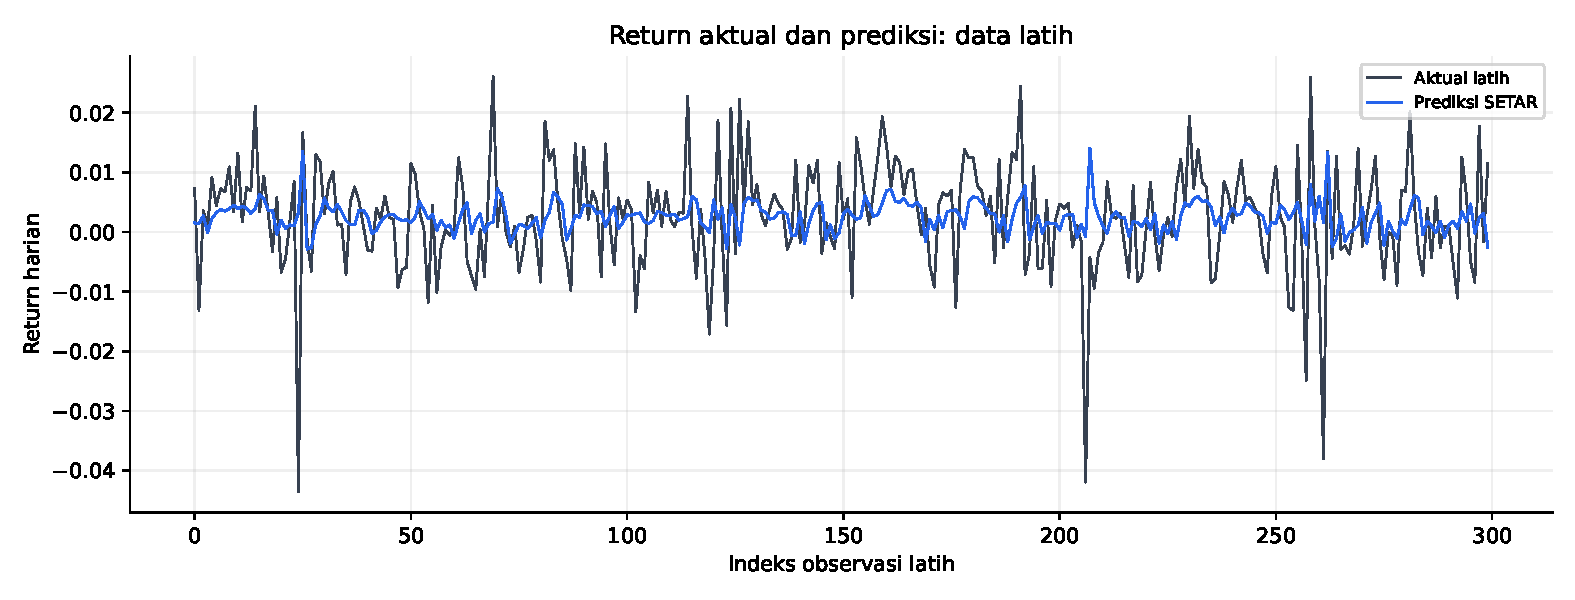
\includegraphics[width=0.82\textwidth]{../soal2/report/figures/train_overlay.pdf}
\caption{Return aktual dan prediksi SETAR pada 300 observasi latih.}
\label{fig:train-overlay}
\end{figure}

\begin{figure}[H]
\centering
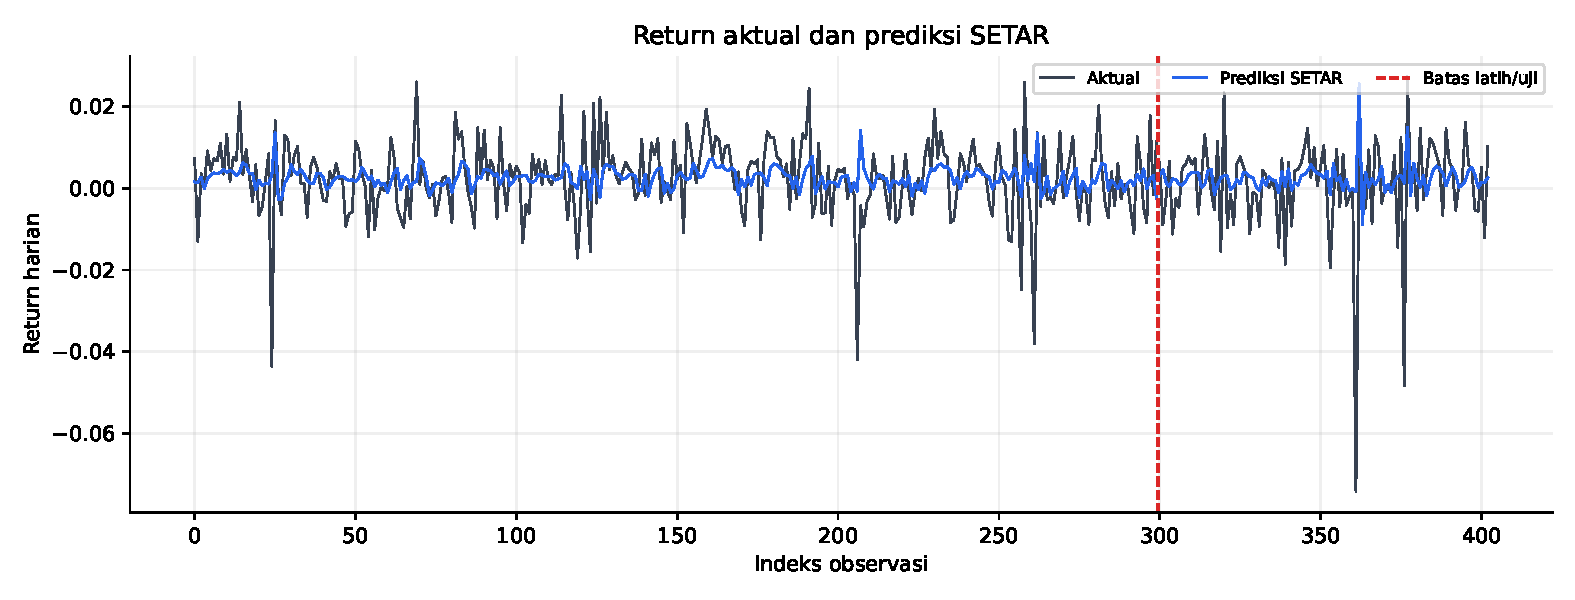
\includegraphics[width=0.82\textwidth]{../soal2/report/figures/overlay.pdf}
\caption{Return aktual dan prediksi dari model yang dilatih pada segmen kiri. Garis putus-putus menunjukkan batas latih/uji; indeks uji pertama memakai riwayat harga latih.}
\label{fig:continuous-overlay}
\end{figure}

\begin{figure}[H]
\centering
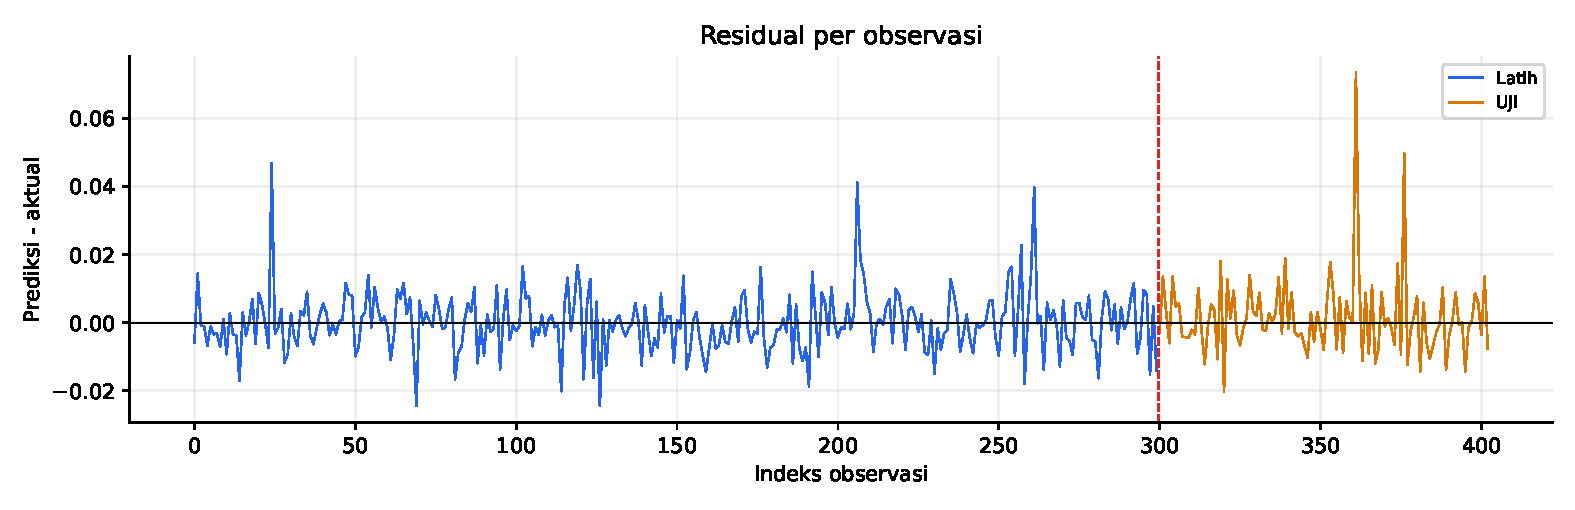
\includegraphics[width=0.82\textwidth]{../soal2/report/figures/residuals.pdf}
\caption{Residual prediksi per observasi. Beberapa deviasi besar tetap muncul walaupun parameter diperoleh dengan meminimalkan jumlah kuadrat galat latih.}
\label{fig:residual}
\end{figure}

\section{Pengaruh outlier}
Gambar~\ref{fig:residual} memperlihatkan galat per observasi, sedangkan Tabel~\ref{tab:outlier} mengukur perubahan setelah observasi ekstrem dihapus.
Fungsi objektif $\sum_t(R_t-\widehat R_t)^2$ memberi bobot kuadrat pada tiap galat. Karena itu kejutan harga ekstrem dapat menaikkan norma residual secara tajam dan menarik koefisien ke arah observasi tersebut. Pada data latih, return absolut terbesar sekitar 0.04357 dan galat prediksi absolut terbesar sekitar 0.04681 (29 Januari 2024). Galat maksimum pada data uji sekitar 0.07347.

Untuk menguji sensitivitas, kami mengestimasi ulang koefisien setelah menghapus satu dan tiga observasi dengan residual terbesar dari data latih, lalu mengevaluasi pada seluruh data latih dan uji yang sama.

\begin{table}[H]
\centering
\caption{Sensitivitas terhadap outlier. Koefisien diestimasi ulang tanpa observasi berresidual terbesar.}
\label{tab:outlier}
\begin{tabular}{lrrr}
\toprule
Metrik & Data penuh & Hapus 1 outlier & Hapus 3 outlier\\
\midrule
RMSE latih & 0.00883213 & 0.00883439 & 0.00884748\\
RMSE uji & 0.01196708 & 0.01200241 & 0.01203210\\
$\norm{x_{\rm penuh}-x_{\rm baru}}$ & --- & $7.62\times10^{-3}$ & $3.03\times10^{-2}$\\
\bottomrule
\end{tabular}
\end{table}

Penghapusan satu outlier (29 Januari 2024) menggeser koefisien rezim bullish---terutama $\phi_{1,1}$ berubah sebesar $+0.0067$---sementara koefisien rezim bearish tidak berubah karena outlier tersebut berada di rezim bullish. RMSE latih dan uji sedikit meningkat karena koefisien baru tidak lagi mengakomodasi observasi ekstrem tersebut. Penghapusan tiga outlier memperbesar pergeseran koefisien empat kali lipat. Hasil ini menunjukkan bahwa satu observasi saja sudah mampu memengaruhi koefisien secara terukur, konsisten dengan sensitivitas kuadrat terkecil terhadap observasi ekstrem.

Kedua solver berhasil menyelesaikan model yang sama dan menghasilkan angka yang identik pada ketelitian pelaporan. Untuk implementasi yang efisien dan lebih tahan terhadap pembulatan, QR Givens sebaiknya diterapkan langsung pada dua baris matriks kerja dan ruas kanan, tanpa membentuk $Q$ atau $G$ dense penuh. Persamaan normal masih layak sebagai pembanding pada data ini, tetapi bilangan kondisinya yang kuadrat perlu diperhatikan jika skala atau korelasi prediktor meningkat.


\section{Kesimpulan}
Persamaan normal dan Givens menghasilkan solusi yang sama sampai presisi yang dilaporkan: norma residual latih $0.15297705$, RMSE latih $0.00883213$, dan RMSE uji $0.01196708$. Pembentukan $A^\mathsf{T}A$ meningkatkan bilangan kondisi dari $192.61$ menjadi $37096.84$; rotasi Givens karena itu lebih aman terhadap pembulatan bila data menjadi lebih buruk kondisinya. Untuk biaya yang wajar, rotasi diterapkan langsung ke dua baris matriks dan ruas kanan tanpa menyimpan $Q$ eksplisit. Koefisien bullish menunjukkan momentum pada kedua lag, sedangkan koefisien bearish menunjukkan pembalikan dalam model ini; akurasi luar sampel lebih rendah daripada akurasi latih.


\noindent\textbf{Reproduksibilitas.} Seluruh langkah komputasi telah dijelaskan dalam dua laporan ini. Program yang digunakan adalah \texttt{soal1/soal1.ipynb} dan \texttt{soal2/program.ipynb}; skrip \texttt{soal2/report/analyze.py} mengulang perhitungan dan grafik SETAR. Ketiganya beserta CSV input dan README disertakan dalam ZIP submisi.

\clearpage
\renewcommand{\refname}{Referensi}
\begin{thebibliography}{9}
\bibitem{norris} J. R. Norris, \emph{Markov Chains}. Cambridge University Press, 1997, Bab 1.3 dan 1.7--1.8.\par
\bibitem{stewart} W. J. Stewart, \emph{Introduction to the Numerical Solution of Markov Chains}. Princeton University Press, 1994.\par
\bibitem{heath} M. T. Heath, \emph{Scientific Computing: An Introductory Survey}, edisi ke-2. McGraw-Hill, 2002, Bab 1--2.\par
\bibitem{lapack} E. Anderson dkk., \emph{LAPACK Users' Guide}, edisi ke-3. SIAM, 1999.\par
\bibitem{gth} W. K. Grassmann, M. I. Taksar, dan D. P. Heyman, ``Regenerative analysis and steady state distributions for Markov chains,'' \emph{Operations Research}, vol. 33, no. 5, hlm. 1107--1116, 1985.\par
\bibitem{golub} G. H. Golub dan C. F. Van Loan, \emph{Matrix Computations}, edisi ke-4. Johns Hopkins University Press, 2013, Bab 5 dan Subbab 5.1.8 (Givens rotations).\par
\bibitem{trefethen} L. N. Trefethen dan D. Bau III, \emph{Numerical Linear Algebra}. SIAM, 1997, Kuliah 11 (least squares), 18 (conditioning of least squares), dan 19 (stability of least squares algorithms).\par
\bibitem{higham} N. J. Higham, \emph{Accuracy and Stability of Numerical Algorithms}, edisi ke-2. SIAM, 2002, Bab 7 dan 20.\par
\end{thebibliography}
\clearpage
\appendix
\renewcommand{\thelstlisting}{A.\arabic{lstlisting}}
\section{Lampiran: Verifikasi dan Rincian Reproduksi}
\subsection{Uji solver untuk Soal 1}
Sebagai uji terukur bagi faktor LU dan permutasi, digunakan
\[
B=\begin{pmatrix}2&1&1\\4&3&3\\8&7&9\end{pmatrix},\qquad
b=\begin{pmatrix}3\\7\\19\end{pmatrix}.
\]
Baris ketiga dipilih sebagai pivot pertama. Dengan urutan baris akhir $(3,1,2)$, kedua implementasi menghasilkan
\[
L=\begin{pmatrix}1&0&0\\1/4&1&0\\1/2&2/3&1\end{pmatrix},\qquad
U=\begin{pmatrix}8&7&9\\0&-3/4&-5/4\\0&0&-2/3\end{pmatrix}.
\]
Perkalian langsung memberi $PB=LU$ dan penyelesaian menghasilkan $z=(1,-1,2)^\mathsf{T}$. Pada uji terpisah, matriks pita $8\times8$ dengan $p=2,q=1$ dan diagonal yang diperkecil 100 kali memicu tujuh pertukaran baris serta delapan elemen \emph{fill-in}; faktor $U$ melebar hingga upper bandwidth $p+q=3$. Ini memeriksa jalur pivot yang tidak terpakai oleh keenam data soal. Pada rantai tiga halte dengan distribusi acuan $(1/4,1/2,1/4)^\mathsf{T}$, kedua solver mengembalikan distribusi tersebut. Uji matriks singular $\left(\begin{smallmatrix}1&2\\2&4\end{smallmatrix}\right)$ ditolak karena pivot akhirnya nol.

\subsection{Nilai rinci dan rotasi pertama untuk Soal 2}
Ada 303 harga latih yang menghasilkan 302 return; setelah dua lag, matriks desain mempunyai 300 baris. Segmen uji mempunyai 103 harga dan 103 return karena return pertama memakai harga penutupan terakhir dari segmen latih. Untuk dua baris pertama desain, $a_{11}=0$ dan $a_{21}=1$, sehingga rotasi pertama mempunyai $c=0$, $s=1$ dan blok $\left(\begin{smallmatrix}0&1\\-1&0\end{smallmatrix}\right)$. Setelah $G_1$ diterapkan, entri $(2,1)$ tepat nol; baris lain tidak berubah pada langkah ini.
\begin{table}[H]\centering\small
\caption{Koefisien SETAR dari QR Givens sebelum pembulatan laporan.}\label{tab:appendix-coeff}
\begin{tabular}{lr}\toprule
Parameter & Nilai\\\midrule
$\alpha_1$ & $0.001513374224392619$\\
$\phi_{1,1}$ & $0.17215289727492178$\\
$\phi_{1,2}$ & $0.16607285095297825$\\
$\alpha_2$ & $-0.0012126885538670722$\\
$\phi_{2,1}$ & $-0.3603768239374077$\\
$\phi_{2,2}$ & $-0.10980803854712604$\\\bottomrule
\end{tabular}\end{table}
Tabel~\ref{tab:appendix-coeff} memuat nilai yang digunakan untuk prediksi tanpa membulatkan koefisien terlebih dahulu. Selisih norma dua antara koefisien persamaan normal dan Givens ialah $2.43949\times10^{-16}$. ZIP submisi menyertakan kedua notebook, delapan CSV input, keluaran eksperimen, dan README dengan langkah menjalankan ulang program.
\clearpage
\subsection{Kode inti dari implementasi}
Kode~\ref{code:soal1} menampilkan bagian faktorisasi kedua solver pada Soal 1. Substitusi segitiga dan normalisasi telah dijabarkan pada Kode~\ref{alg:soal1-solvers}; implementasi lengkap disertakan dalam notebook. Kode~\ref{code:soal2} menampilkan solver persamaan normal dan Givens dari skrip reproduksi Soal 2. Rotasi diterapkan langsung pada dua baris matriks kerja dan ruas kanan, lalu diakhiri substitusi balik.
\lstinputlisting[caption={Faktorisasi LU dense dan pita pada Soal 1.},label={code:soal1}]{code_soal1.py}
\clearpage
\lstinputlisting[caption={Solver Gauss berpivot dan QR Givens pada Soal 2.},label={code:soal2}]{code_soal2.py}
\end{document}
